\chapter{Reflectance Measurements of Road Materials}

Road surfaces are inherently heterogeneous owing to variations in material composition, aging, weathering, and surface texture.
These variations cause spatial and temporal changes in reflectance characteristics that influence both the visual performance of lighting installations and the thermal behavior contributing to urban heat island effects.
To better understand these changes, numerous field and laboratory optical measurements of road surface materials have been conducted in recent decades, focusing mainly on BRDF~\cite{1995_Oren,2000_Meister,2010_Roser,2023_Spieringhs} and solar albedo~\cite{1988_Blumthaler,2011_KUSHARI,2019_Chen,2022_Bai}.
The former quantifies the angular distribution of reflected light, which is critical for optimizing visibility, and the latter represents the fraction of solar reflected radiation which governs pavement thermal performance.
This chapter provides the overview of the measurements conducted in the past twenty years in terms of BRDF and solar albedo of different materials of roads.

%%%%%%%%%%%%%%%%%%%%%%%%%%%%%%%%%%%%%%%%%%%%%%%%%%%%%%%%%%%
\section{BRDF Measurements of Road Materials}

In road surface analysis, BRDF measurements offer a detailed understanding of surface reflectance properties, that impacts not only human safety but also the performance of automated systems, such as LiDAR and camera-based sensors in autonomous vehicles.


%%%%%%%%%%%%%%%%%%%%%%%%%%%%%%%%%%%%%%%%%%%%%%%%%%
\subsection{BRDF Measurement Set-up}

The BRDF measurement systems for road surface can be broadly categorized into two types: laboratory-based and field-based approaches.
The former is typically conducted under controlled environments where factors such as lighting, geometry, and surface conditions can be precisely controlled.
The classic laboratory-based systems, such as gonioreflectometer~\cite{1995_Oren,2022_Hebert,2023_Spieringhs} and gonio-spectroradiometer if the detection is spectral~\cite{2000_Meister,2022_Wise, 2023_Zhuang}, observe the same surface sample under varying observer and light source position, as seen in Fig~\ref{fig:lab-measure}.
They are commonly composed of the goniometer used to change the angles of incidence and detection (e.g.by rotating the robot swing arms~\cite{1995_Oren,2022_Hebert,2022_Wise}, as seen in Fig~\ref{fig:gonio-oren} and Fig~\ref{fig:gonio-swing}), the light source and the detection sensors (e.g. camera, spectroradiometer).
In many studies, halogen lamp is used as the light source due to its spectrum close to solar spectrums~\cite{2000_Meister,2022_Hebert, 2023_Spieringhs,2022_Wise,2023_Zhuang}.

\begin{figure}[!tb]
    \centering
    \subfigure[Gonioreflectometer using a long beam]{
        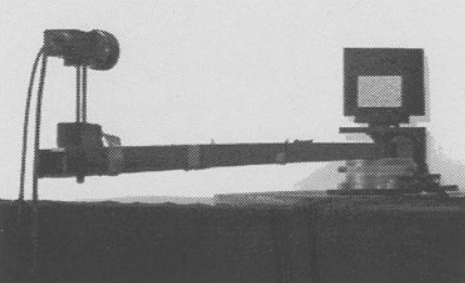
\includegraphics[width=0.45\linewidth]{./figures/optical-properties-of-road-surface/gonio-oren.png}
        \label{fig:gonio-oren}
    }
    \hfil
    \subfigure[Large near-field gonioreflectometer]{
        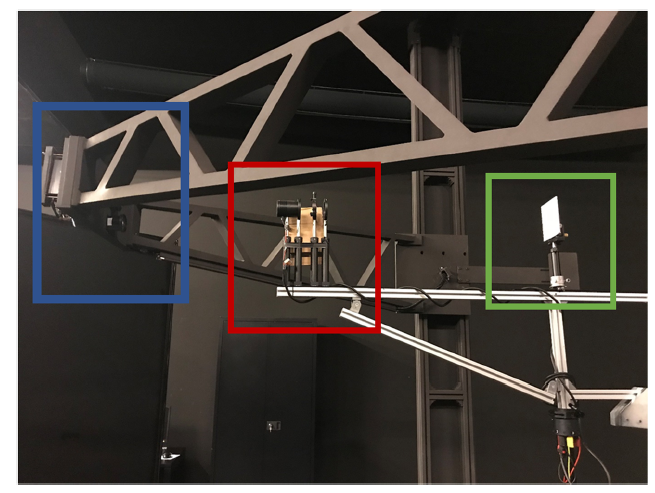
\includegraphics[width=0.45\linewidth]{./figures/optical-properties-of-road-surface/gonio-tech.png}
        \label{fig:gonio-tech}
    }
    \hfil
    \subfigure[Gonio-spectroradiometer using 2 swing arms]{
        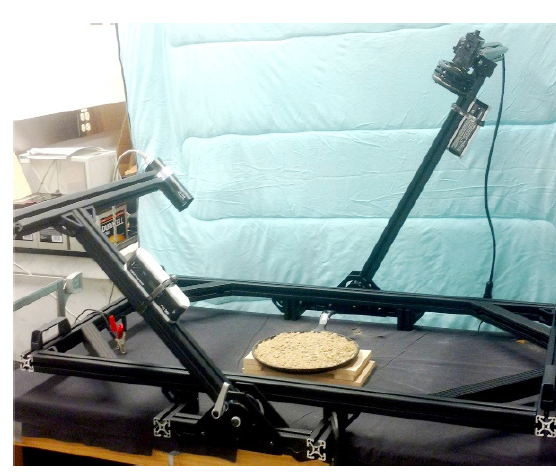
\includegraphics[width=0.45\linewidth]{./figures/optical-properties-of-road-surface/gonio-swing.png}
        \label{fig:gonio-swing}
    }
    \hfil
    \subfigure[Gonio-spectroradiometer using two bars]{
        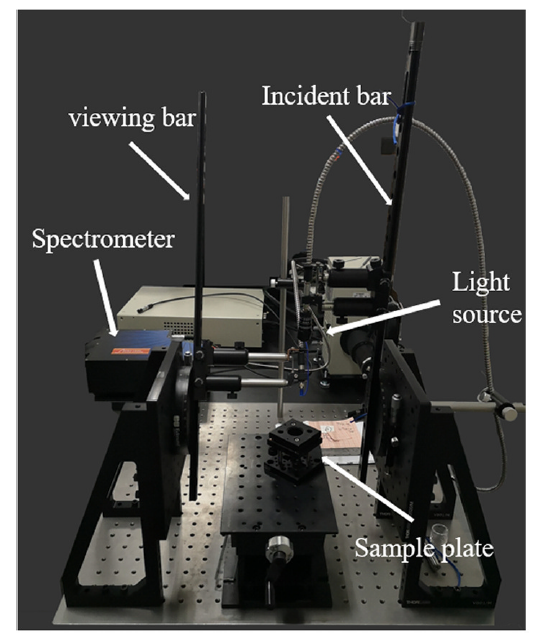
\includegraphics[width=0.45\linewidth]{./figures/optical-properties-of-road-surface/gonio-bidirection.png}
        \label{fig:gonio-bars}
    }
    \caption{BRDF Laboratory measurement set-up}
    \label{fig:lab-measure}
\end{figure}

The latter is essential to obtain realistic data of road surface BRDF under actual environmental conditions, such as varying sunlight (from sunrise to sunset), weather (e.g. sunny, cloudy, rainy), and surface states (dry or wet).
An example of such a setup is vehicle-based automotive measurement systems~\cite{2010_Roser} (see in Fig~\ref{fig:automotive-set-up}), where natural sunlight serves as the light source and detection sensor, such as camera, is mounted on the car's front window.
Apart from this set-up, the lab-based set-up presented in Fig~\ref{fig:gonio-swing} is extended to measure the soil surface outside~\cite{2022_Wise} by digging a small trench so that the pivot point of the pendulum arm coincided with the soil surface, as shown in Fig~\ref{fig:gonio-filed-measure}

\begin{figure}[!tb]
    \centering
    \subfigure[Vehicle-Mounted set-up]{
        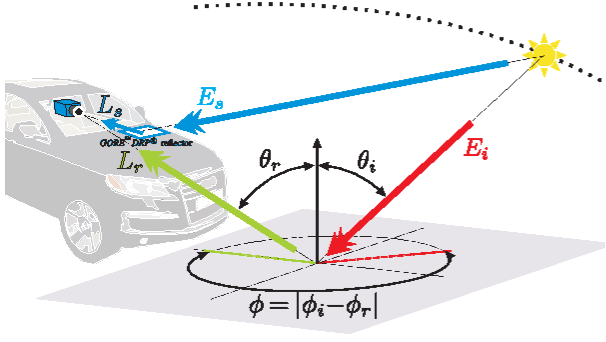
\includegraphics[width=0.45\linewidth]{./figures/optical-properties-of-road-surface/automotive-setup.png}
        \label{fig:automotive-set-up}
    }
    \hfil
    \subfigure[Gonioreflectometer using 2 swing arms]{
        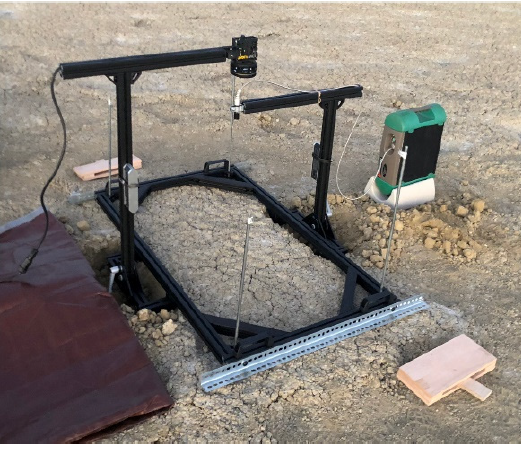
\includegraphics[width=0.45\linewidth]{./figures/optical-properties-of-road-surface/field-setup.png}
        \label{fig:gonio-filed-measure}
    }
    \caption{BRDF Field-based measurement set-up}
    \label{fig:field-based-measure}
\end{figure}



%%%%%%%%%%%%%%%%%%%%%%%%%%%%%%%%%%%%%%%%%%%%%%%%%%
\subsection{Former work on BRDF Measurement of Different Road Materials}

In practical applications, road surfaces like asphalt and concrete are commonly made from a combination of aggregates and binders.
The optical properties of these road materials have been extensively studied to support accurate modeling.
To evaluate the accuracy of their diffuse reflectance model developed in 1993~\cite{1995_Oren}, Oren and Nayar conducted several experiments restricted to the visible spectrum, using road-like materials as test samples, such as plaster and white sand.
Their experiment set-up is given in Fig~\ref{fig:gonio-oren}, where a $512\times 480 $ pixel charged-coupled device (CCD) camera as receiver is mounted at the end of a 6 foot long beam and $300 $ Watt incandescent light source is used to illuminate the sample.
A pair of fitting parameters of their BRDF model (ON Model as described in Section~\eqref{subsec: oren-nayar-model}), diffuse albedo $\rho$ and surface roughness $\sigma$ were empirically chosen to obtain the best fit with the measured radiance.
The optimal parameter values were found to be $\rho = 0.9$, $\sigma = 30^\circ$ for plaster, and $\rho = 0.8$, $\sigma = 35^\circ$ for white sand, as shown in Fig~\ref{fig:ON-fitting-plaster} and Fig~\ref{fig:ON-fitting-white-sand} respectively.
In both figures, the solid lines and the dotted points respectively show the radiance predicted by ON model and the measured radiance.
Notice that these measurements were made in the plane of incidence ($\varphi_r =\varphi_i$ and $\varphi_r =\varphi_i +\pi$ corresponding to negative and positive values of $\theta_r$).
For both plaster and white sand, the measured radiance shows a clear peak in the specular direction, where the this model exhibits poor fitting performance.
This indicates that ON model is not well-suited for capturing specular reflectance.

\begin{figure}[!tb]
    \centering
    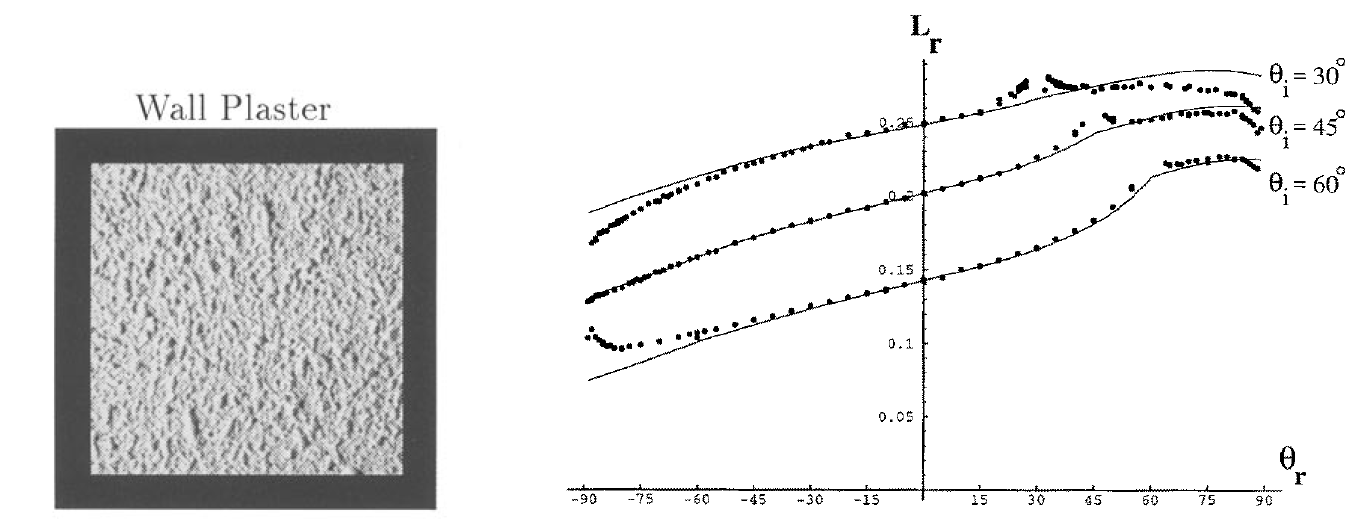
\includegraphics[width=0.9\linewidth]{./figures/measurement-literature/ON-fitting-plaster-full.png}
    \caption{Plaster: Oren Nayar model fitting to measured radiance}
    \label{fig:ON-fitting-plaster}
\end{figure}

\begin{figure}[!tb]
    \centering
    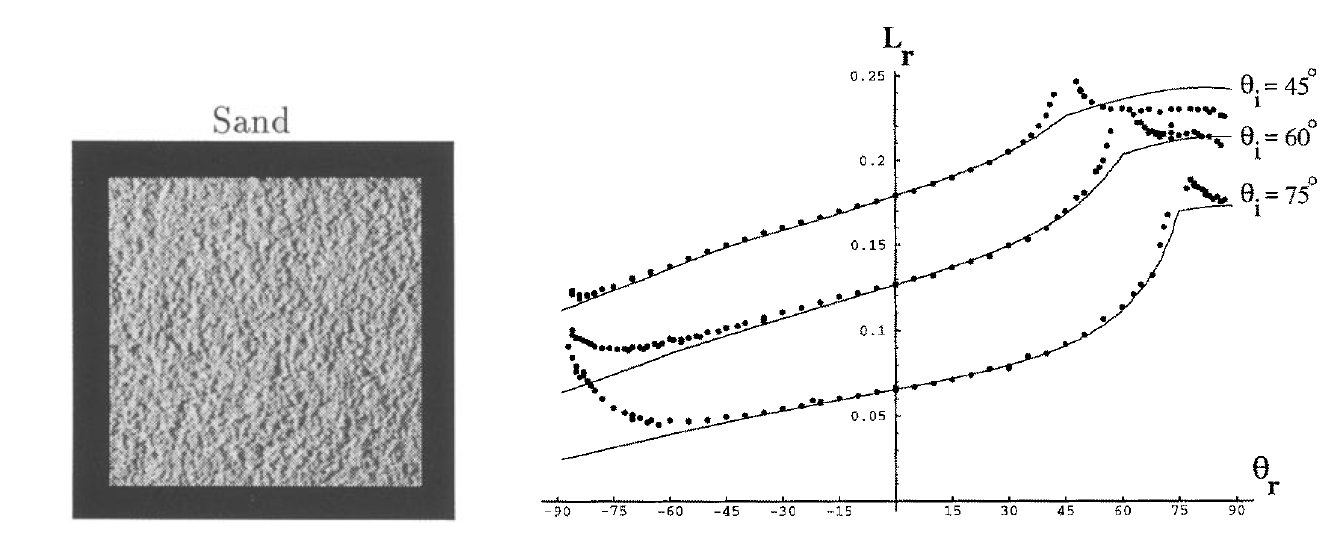
\includegraphics[width=0.9\linewidth]{./figures/measurement-literature/ON-fitting-white-sand-full.png}
    \caption{White sand: Oren Nayar model fitting to measured radiance}
    \label{fig:ON-fitting-white-sand}
\end{figure}

To compensate for this deficiency, Meister extended ON model by linearly combining it with a specular reflectance model (TS model as described in Section~\eqref{subsec:brdf-cook-torrance}) to fit spectral BRDF measurement for asphalt respectively at $425nm$ and $660nm$ over the period from 1995 to 2000~\cite{2000_Meister}, as illuminated in Fig~\ref{fig:ON-fitting-asphalt}.
In addition, he also applied a mixed model which linearly combined Lambertian model and TS model to fit the measured spectral BRDF of blue/red concrete respectively at the same wavelength, as shown in Fig~\ref{fig:CT-fitting-blue-concrete} and Fig~\ref{fig:CT-fitting-red-concrete}.
These measurements were performed at the European Goniometric Facility (EGO) in Italy using a specially designed goniometer.
Instead of employing a rotating robotic arm used by Oren and Nayar, this goniometer is constructed using two quarter arcs with a radius of 2 meters, which allow for the flexible mounting of a sensor and a light source~\cite{2000_Meister}.
To measure the spectral BRDF, this setup was modified by replacing the camera with an SE590 spectroradiometer, capable of capturing wavelengths in the range of 400 nm to 1100 nm.
A $1000$-watt halogen lamp was used as the light source due to its spectral similarity to sunlight.
As observed from Fig~\ref{fig:ON-fitting-asphalt} to Fig~\ref{fig:CT-fitting-red-concrete}, the measured BRDFs were well fitted across most configurations.

\begin{figure}[!tb]
    \centering
    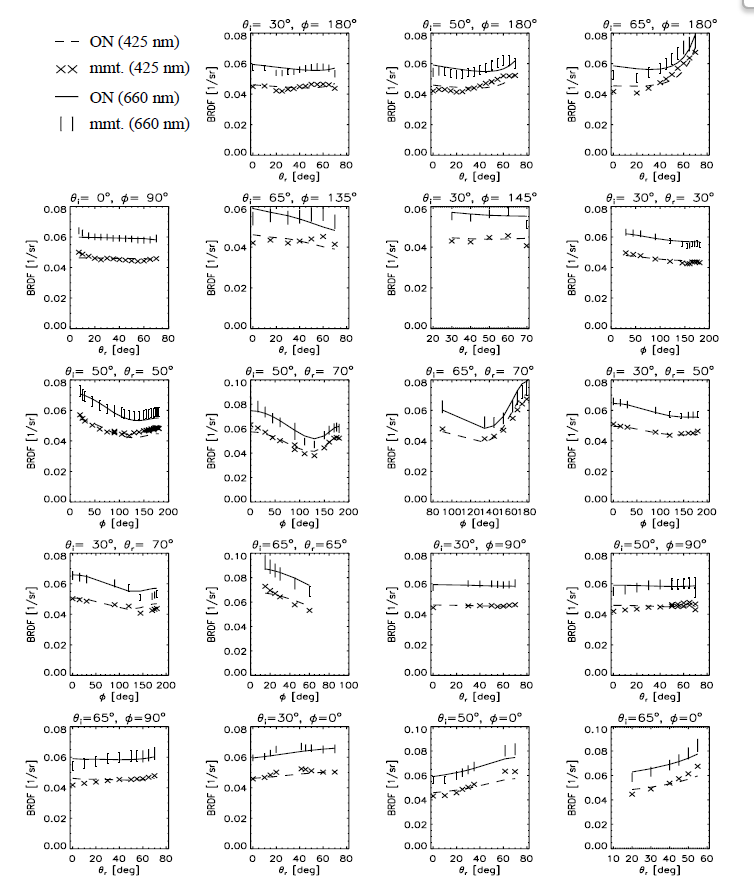
\includegraphics[width=0.9\linewidth]{./figures/measurement-literature/ON-fitting-asphalt.png}
    \caption{Asphalt: mixed reflectance model (ON + CT) fitting to measured BRDF}
    \label{fig:ON-fitting-asphalt}
\end{figure}

\begin{figure}[!tb]
    \centering
    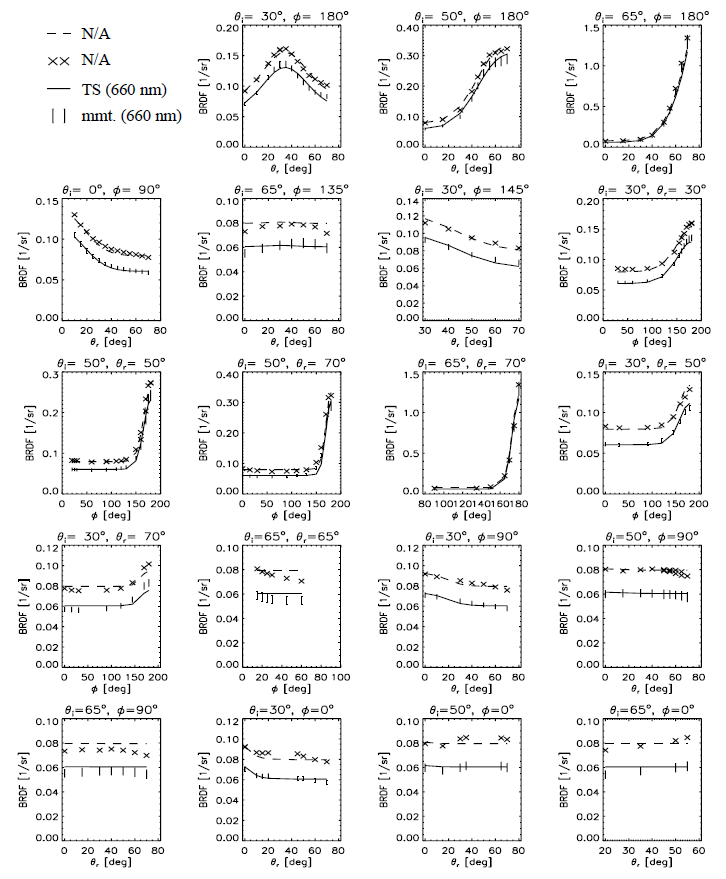
\includegraphics[width=0.9\linewidth]{./figures/measurement-literature/CT-fitting-blue-concrete.png}
    \caption{Blue concrete: mixed reflectance model (Lambertian + CT) fitting to measured BRDF}
    \label{fig:CT-fitting-blue-concrete}
\end{figure}

\begin{figure}[!tb]
    \centering
    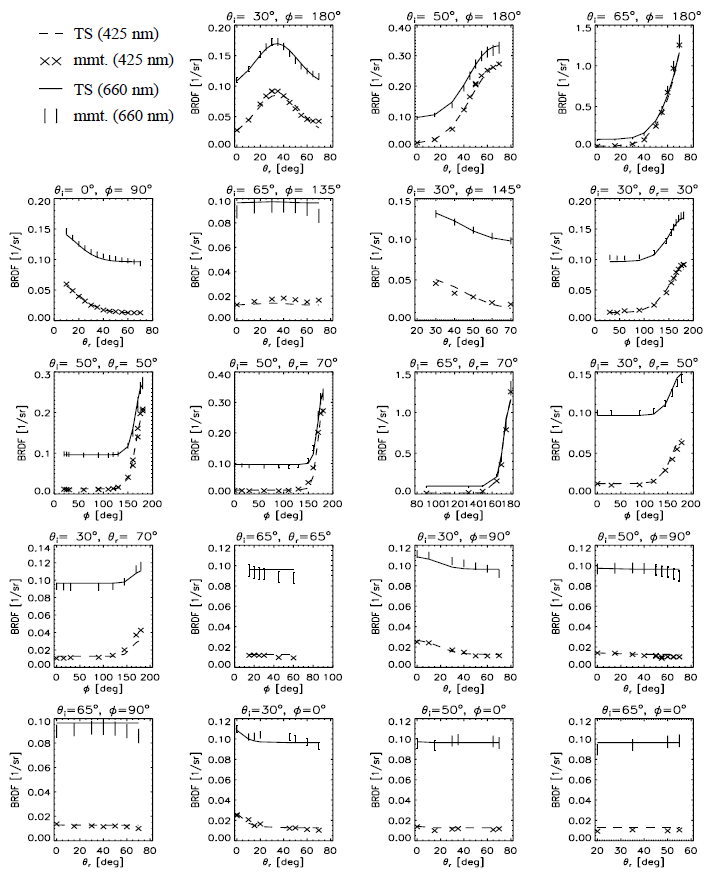
\includegraphics[width=0.9\linewidth]{./figures/measurement-literature/CT-fitting-red-concrete.png}
    \caption{Red concrete: mixed reflectance model (Lambertian + TS) fitting to measured BRDF}
    \label{fig:CT-fitting-red-concrete}
\end{figure}

In addition to the laboratory-based setup, Roser et al. conducted several experiments directly on natural concrete road surfaces using a three-dimensional geometric model of the automotive BRDF measurement system~\cite{2010_Roser}, as shown in Fig~\ref{fig:field-based-measure}.
The camera with known orientation was mounted behind the windshield, and sunlight was serving as the sole source of illumination.
This system leverages single grayscale images, integrated with GPS and vehicle heading data, to estimate the reflectance properties of small road patches under both dry and damp conditions.
The resulting measured data were subsequently fitted using the extended ON reflectance model that is same as the one used by Meister, as seen in Fig~\ref{fig:ON-fitting-road-concrete}.
This extended model and their parameters were able to successfully differentiate between different pavement reflection conditions.

\begin{figure}[!tb]
    \centering
    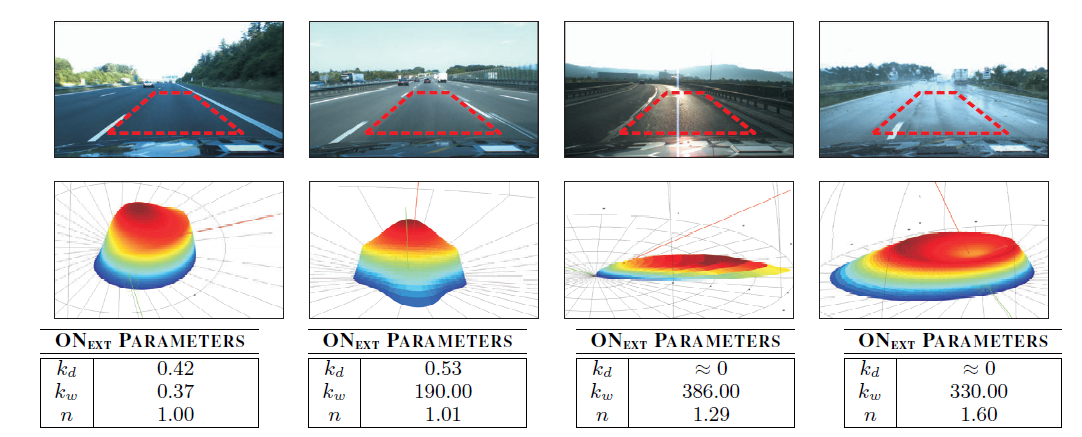
\includegraphics[width=0.9\linewidth]{./figures/measurement-literature/ON-fitting-road-concrete.png}
    \caption{Concrete road: mixed reflectance model (ON + TS) fitting to measured BRDF}
    \label{fig:ON-fitting-road-concrete}
\end{figure}

In recent years, Wise et al. conducted extensive measurements on beach sands under darkened conditions\cite{2022_Wise}, using a goniometer-based setup shown in Fig.\ref{fig:gonio-swing} that was transitioned to field use as illuminated in Fig~\ref{fig:gonio-filed-measure}.
A spectroradiometer covering the $400-2400nm$ range and a halogen lamp were employed in their experiments,  and were mounted on a portable, manually operated goniometer constructed from aluminum struts.
In this goniometer design, the platform at the base measured $122 \times 61$cm and supported two swing arms, measuring $46cm$ and $66cm$ in length, with a total system weight of approximately $9kg$.
It allows for measuring the spectral BRDF over a 140-degree range ($-70^\circ$ - $70^\circ$) to within 3 degrees of backscatter.
These measured BRDF data were fitted using Hapke's SHOE model described in Section~\eqref{sec:brdf-Hapke} wherein a series expansion of Legendre Polynomials was substituted for the angularly dependent backscatter function.
The best-fit model BRDF was then integrated over the hemisphere to compute the Directional Hemispheric Reflectance (DHR), as shown in Fig~\ref{fig:hapke-fitting-sand}.
It can be observed that the integrated Lab BRDF (black) is almost overlapped with the measured DHR (blue), verifying the effectiveness of this BRDF model in capturing reflectivities of beach sands.

\begin{figure}[!tb]
    \centering
    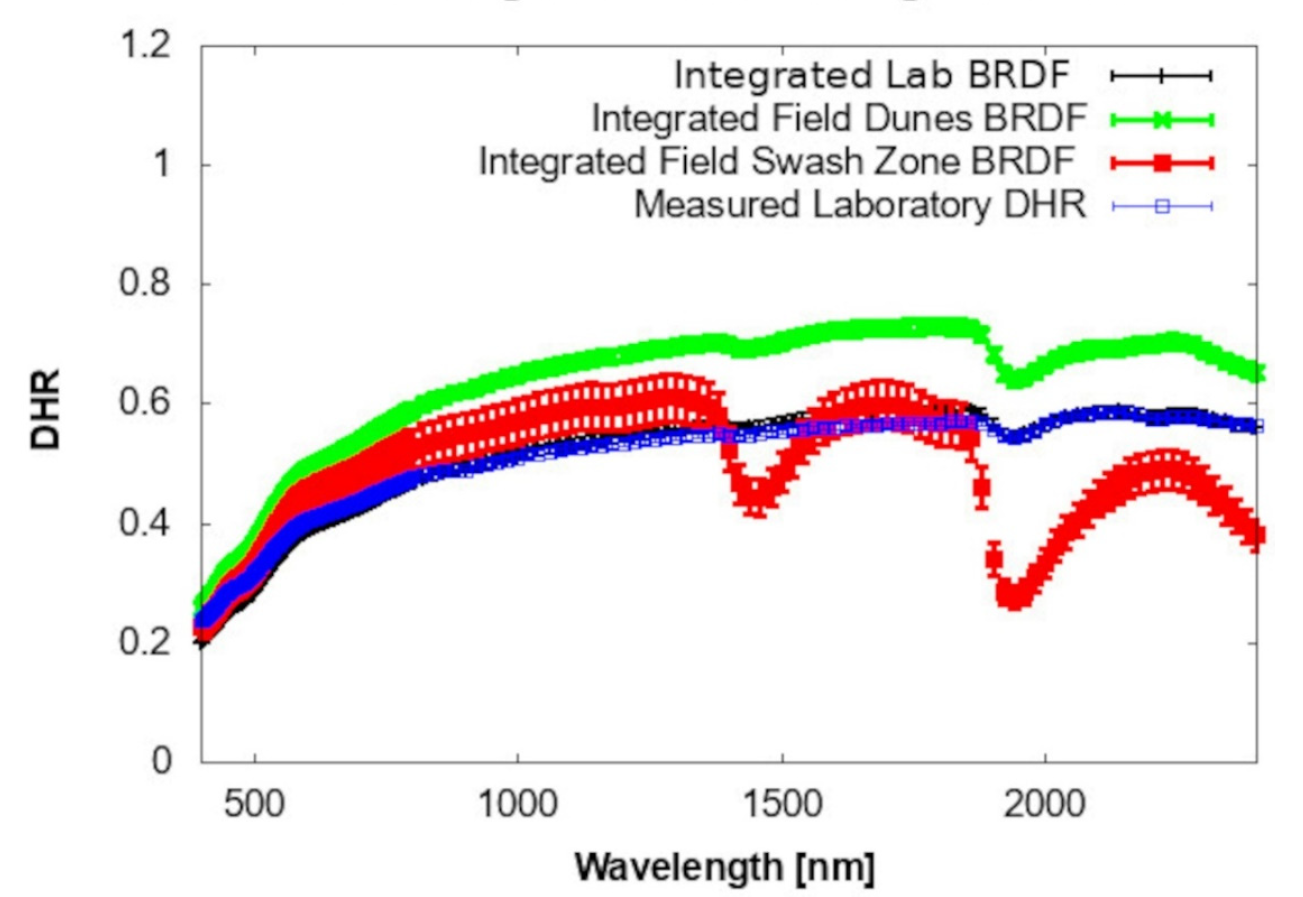
\includegraphics[width=0.9\linewidth]{./figures/measurement-literature/hapke-fitting-island.png}
    \caption{Chincoteague Island beach sand: Hapke's SHOE model fitting to measured DHR}
    \label{fig:hapke-fitting-sand}
\end{figure}

Apart from the beach sands, many spectral reflectance measurements on 13 different igneous rocks (seen in Fig.\ref{fig:rocks}) and their powders with different sizes in visible and near-infrared range from $400nm$ to $2500nm$ were performed by Zhuang et al.~\cite{2023_Zhuang}.
Similar to the experimental set-up in~\cite{2022_Wise},  the spectrometer and the light source were mounted on manually operated goniometer that consists of two rotary stages with bars, as shown in Fig~\ref{fig:gonio-bars}.
This set-up design is capable of adjusting the viewing and the incident zenith angles from $0^\circ$ to $70^\circ$ continuously.
To emit the spectrum from $400nm$ to $2500nm$, the light source they utilized was highly stable Newport 66502-250Q-R1 quartz tungsten halogen lamp with an adjustable power range from 0-250W.
The reflected light is collected by a bare fiber and transmitted to Spectral Evolution SR-2500 spectrometer.
In their work, they measured respectively the intensities from the target sample and the reference Lab-sphere Spectralon plaque at incident zenith angle of $0^\circ$ and a viewing zenith of $30^\circ$.
Their ratio was considered as the relative reflectance, which is used to compute the reflectance factor (REFF) of this sample by multiplying the absolute Spectralon REFF values measured by RELAB~\cite{2023_Zhuang}.
These measurements were then fitted also using the Hapke's SHOE model, where the phase function is approximated by an empirical two-term Legendre polynomial.
As illustrated in Fig~\ref{fig:hapke-fitting-rocks}, the fitted spectral reflectance curves for some samples with particle sizes exceeding $675\mu m$ are too similar to be clearly distinguished.
It can also be observed that this model may not produce accurate spectral reflectance for all samples and particle sizes, likely due to its inherent simplicity and the assumption of a constant refractive index ($n = 1.6$) irrespective of wavelengths.

\begin{figure}[!tb]
    \centering
    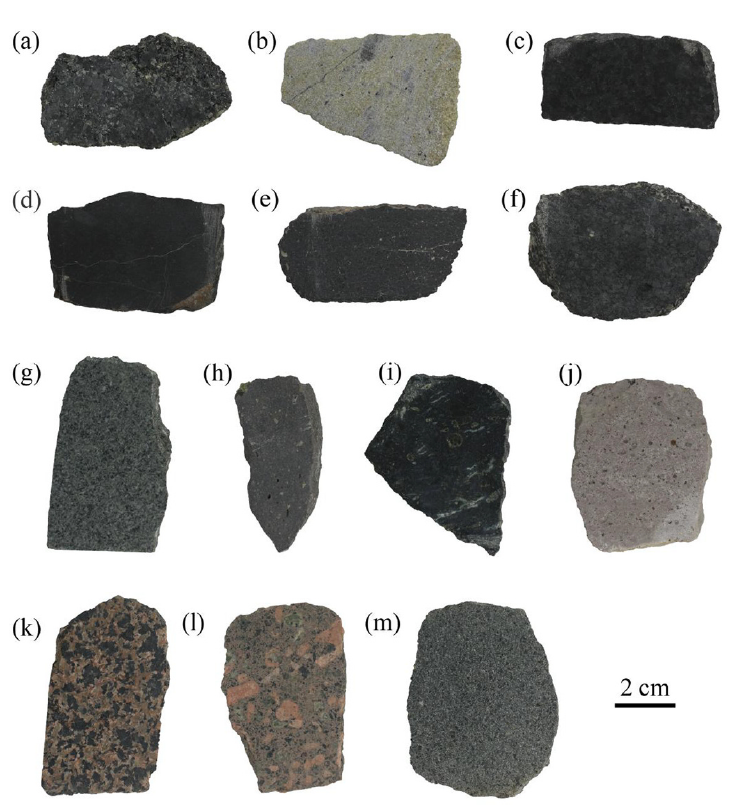
\includegraphics[width=0.9\linewidth]{./figures/measurement-literature/rocks-slab.png}
    \caption{13 igneous rocks slabs with a thickness of 1.5 cm: (a) Dunite; (b) Peridotite; (c) Olivine
        pyroxenolite; (d) Picrite porphyrite; (e) Kimberlite; (f) Gabbro; (g) Diabase; (h)
        Olivine basalt; (i) Andesite basalt; (j) Trachyte; (k) Pyroxenite syenite; (l)
        Orthophyre; (m) Lamprophyre.}
    \label{fig:rocks}
\end{figure}

\begin{figure}[!tb]
    \centering
    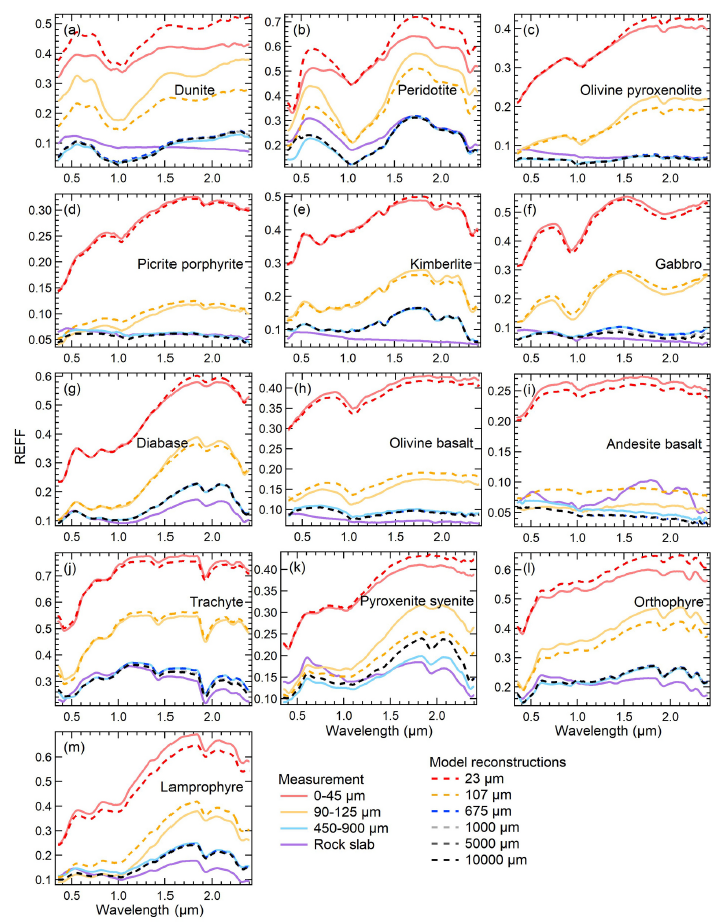
\includegraphics[width=0.9\linewidth]{./figures/measurement-literature/hapke-fitting-rocks.png}
    \caption{Igneous rocks: Hapke's SHOE model fitting to measured REFF}
    \label{fig:hapke-fitting-rocks}
\end{figure}


Alongside studies on road materials, the optical properties of road markings have attracted increasing attention in recent years.
Spieringhs et al.\cite{2023_Spieringhs} carried out several experiments on three different types of road markings (seen in Fig~\ref{fig:3-road-markings}) using a Large Near-Field Goniometer (LNFG) developed by TechnoTeam, as shown in Fig.\ref{fig:gonio-tech}.
The elements highlighted in blue, red, and green boxes correspond to the luminance camera, the fixed light source, and the sample holder, respectively.
In their measurements, a TechnoTeam LMK 98-4 high-tech calibrated luminance camera with a resolution of $1390\times1040$ pixels was mounted in the RIGO801 LNFG, which can be moved freely in order to allow for measurements in all desired viewing angles.
Then the camera and the RIGO801 LNFG are connected to the computer in order to set the position of the arm of the LNFG via the TechnoTeam software and to record the luminance images.
A QTH10(/M) Quartz Tungsten-Halogen $50W$ $12V$ lamp with a broadband emission between $400$ and $2200 nm$ was employed as light source and connected to programmable Delta Elektronika SM1500 DC power system.
Notice that the position of light source is fixed, indicating that it is impossible to allow for all desired incident angles ($\theta, \varphi$) by changing the position of light source.
To accommodate this, an adjustable sample holder was designed to enable rotation around both vertical and horizontal axes.
These measured data for 3 road markings were shown  in Fig~\ref{fig:measured-3-road-markings}.
As the incident angle $\theta_i$ increases, retro-reflection and specular reflection become more pronounced.
Particularly at $\theta_i = 80^\circ$, the BRDF in the retro-direction nearly reaches or exceeds 1.
To able to predict the BRDF at any incident angles ($\theta_i, \varphi_i$) and viewing angles ($\theta_r, \varphi_r$), the authors employed the retro-phong model (described in Section~\eqref{sec:brdf-retro-phong}) to fit the measurements.
A fitting example for road marking sample 1 was presented in Fig~.\ref{fig:retor-phong-fitting-road-marking}.
Compared to the other models evaluated in~\cite{2023_Spieringhs}, this model demonstrated better fitting performance.

\begin{figure}[!tb]
    \centering
    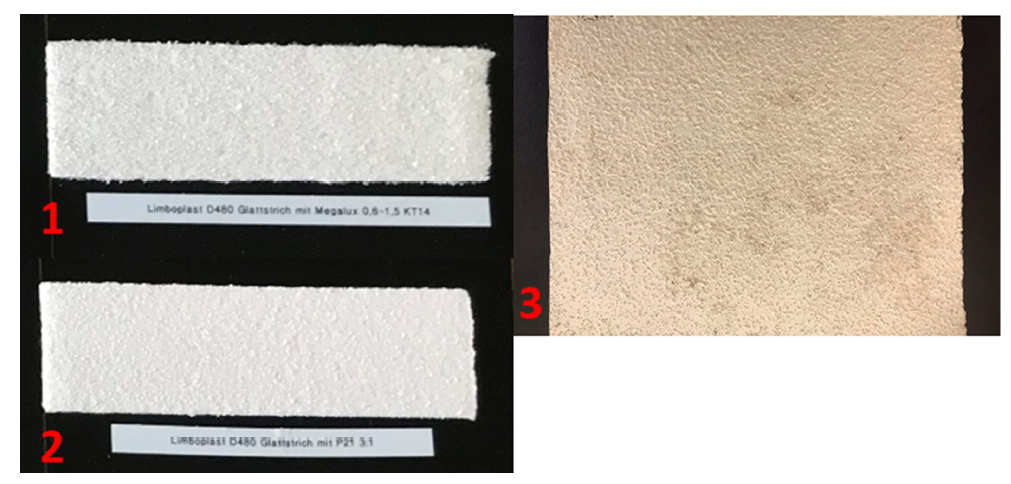
\includegraphics[width=0.9\linewidth]{./figures/measurement-literature/3-road-markings.png}
    \caption{Three road marking samples containing glass beads: (1) SWARCO Limboplast $D480$ withMegalux $0.6-1.5$ KT14, (2) SWARCO Limboplast D480 with $P21$ $3:1$, and (3)3MStamark $A650$.}
    \label{fig:3-road-markings}
\end{figure}

\begin{figure}[!tb]
    %\centering
    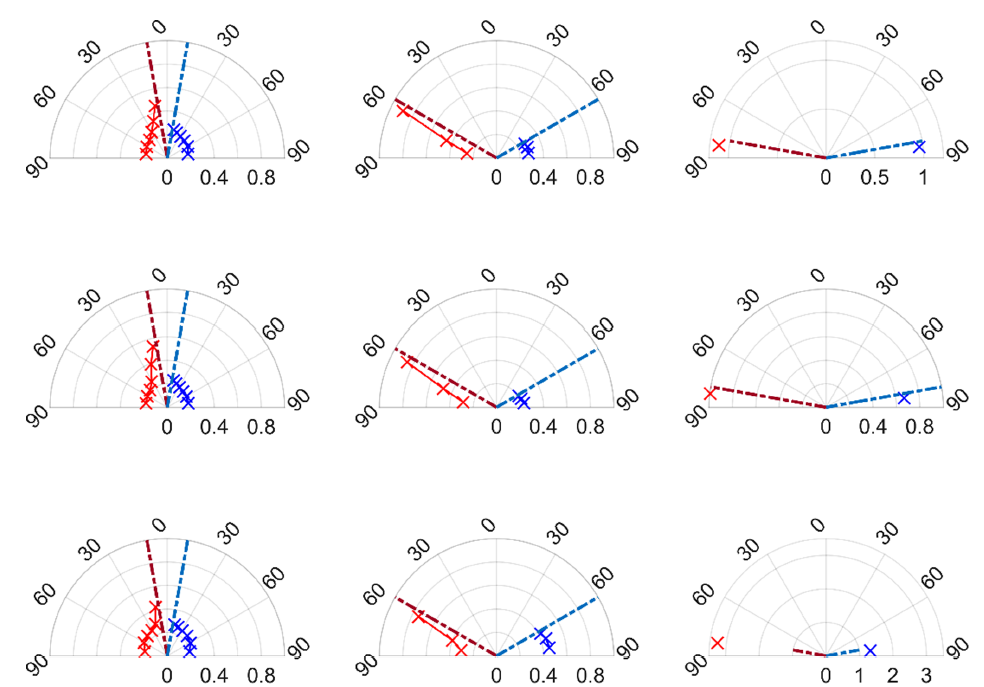
\includegraphics[width=0.9\linewidth]{./figures/measurement-literature/measured-3-road-markings.png}
    \caption{Measured BRDF: Top row for sample 1, middle row for sample 2, bottom row for sample 3.
        The 3 plots in a row represent an incident angle of $\theta_i = 0^\circ, 60^\circ, 80^\circ$ for a fixed $\varphi_i$} from left to right, respectively.
    The crosses and dashed lines in red represent the retro-reflective hemisphere, and the ones in blue represent the specular hemisphere.
    The red dotted lines indicate the incident vectors.
    The radius of the polar diagrams is in $sr^\circ$.
    \label{fig:measured-3-road-markings}
\end{figure}

\begin{figure}[!tb]
    \centering
    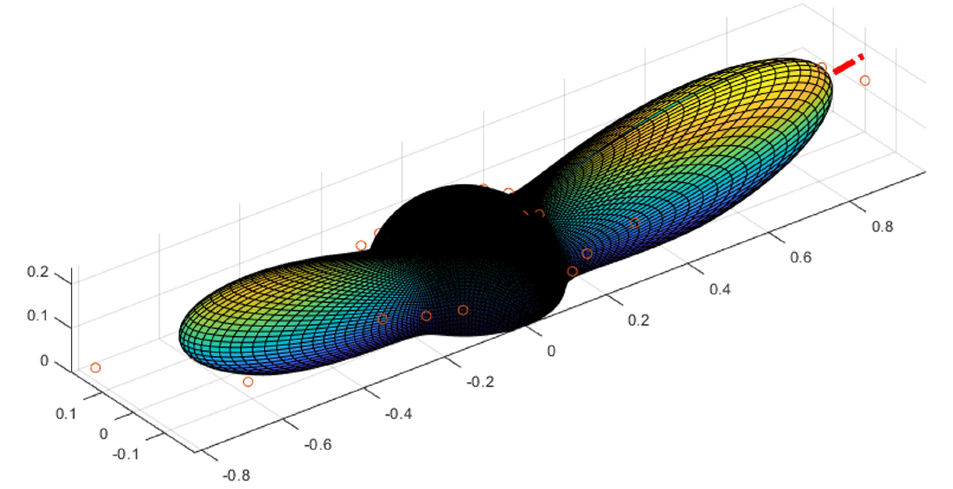
\includegraphics[width=0.9\linewidth]{./figures/measurement-literature/retro-phong-fitting-road-marking-1.png}
    \caption{Road marking sample 1 (SWARCO Limboplast $D480$ withMegalux $0.6-1.5$ KT14): Retro-Phong model fitting to measured BRDF.
        The dashed lines indicate the incident direction, the colored grids represent the fitted BRDF, the dots indicate the measured BRDFs in different viewing angles}
    \label{fig:retor-phong-fitting-road-marking}
\end{figure}

%%%%%%%%%%%%%%%%%%%%%%%%%%%%%%%%%%%%%%%%%%%%%%%%%%%%%%%%%%%
\section{Solar Albedo Measurements of Road Materials}

%%%%%%%%%%%%%%%%%%%%%%%%%%%%%%%%%%%%%%%%%%%%%%%%%%
\subsection{Albedo Measurement set-up}

Similar to BRDF measurements, there exist two primary approaches of measuring solar albedo: laboratory-based and field-based measurements.~\cite{2019_Chen}.
The former is carried out indoors using a spectrophotometer equipped with integrating spheres, as following the standard test ASTM E903.
The goal is to obtain the spectral reflectance which is an approximate estimate of solar albedo.
This kind of test method is applicable to materials having both specular and diffuse optical properties.

\begin{figure}[!tb]
    \centering
    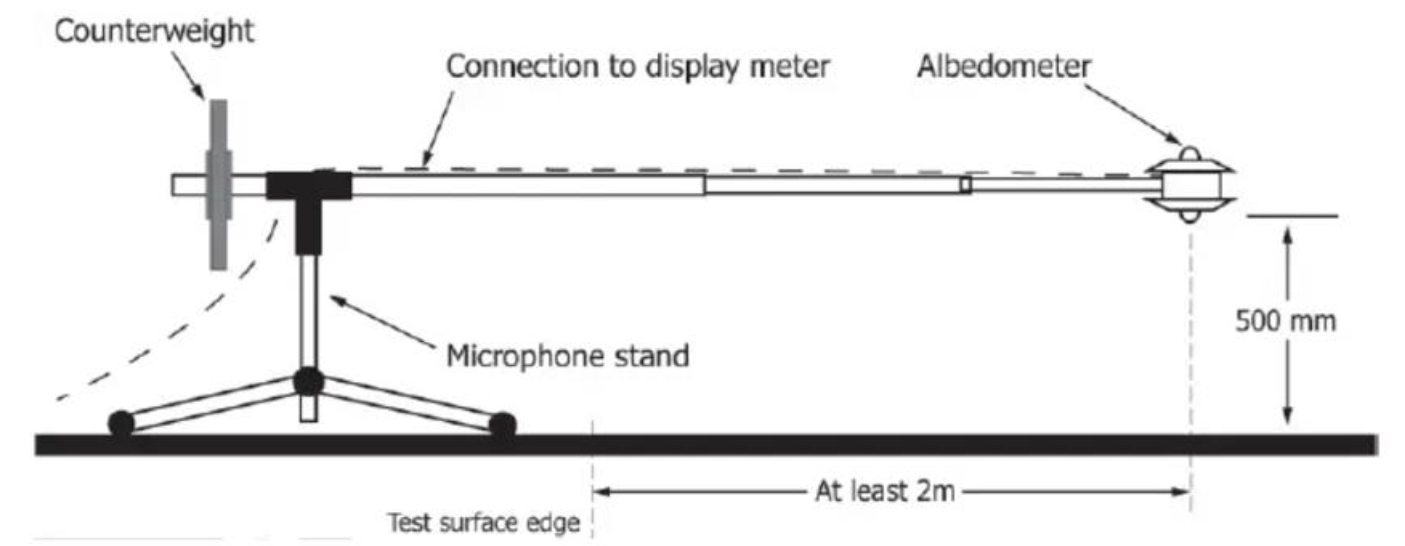
\includegraphics[width=0.9\linewidth]{./figures/optical-properties-of-road-surface/albedometer.png}
    \caption{Schematic of the Albedometer and Its Support (provided in ASTM 1918-21)}
    \label{fig:albedometer}
\end{figure}

While the latter is following ASTM 1918, providing an realistic measure of solar albedo, but highly depending on the weather conditions.
It is conducted outside using an albedometer composing of sky-facing and target-facing pyranometers parallel to the test surface, as seen Fig~\ref{fig:albedometer}, which are used to measure the incoming and reflected solar radiation respectively.
The two pyranometers are mounted on an arm and a stand that centers the sensor at a height of $500mm$ above the target surface in order to minimize the effects of sensor, arm, and stand shadows on measured reflected radiation.
The horizontal distance from the center of the pyranometer to the edge of the test surface has to be at least $2m$.
Besides, the arm and stand should be strong and cast the smallest possible shadow.
This test method applies to low-sloped surface which are at least $4m$ in diameter (if circular) or at least $4m$ on each side (if rectangular).
Notice that the angle of the sun to the normal of the test surface should be less than $45^\circ$.
Due to horizontal and low-sloped surfaces, the hours in summer for this test should be between $9.a.m$ and $3.p.m$ local standard time, which is when solar radiation is at least $70\%$ of the value obtained at noon for that day.
In winter, conducting the test should be between $10.a.m$ and $2.p.m$ local time, considering low solar incident angle.
The albedometer will read both the incoming solar radiation and the reflected solar radiation simultaneously.
To ensure the accuracy, each reading should be constant for at least $10s$ before recording the its values.
Plus, at least $3$ pairs of incoming and reflected radiation are required to be measured within $2$ minutes.
The calculated solar reflectance which is the ratio of the reflected radiation to the incoming radiation need to agree to within $0.01$ in a reflectivity scale of $0$ to $1$.

\begin{figure}[!tb]
    \centering
    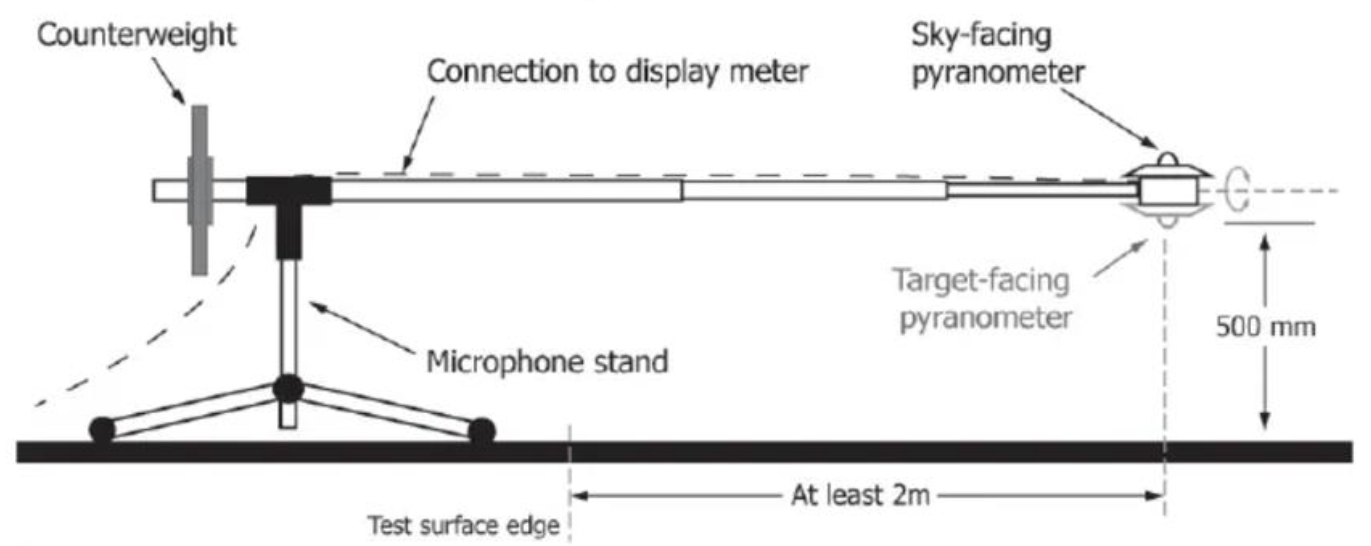
\includegraphics[width=0.9\linewidth]{./figures/optical-properties-of-road-surface/pyranometer.png}
    \caption{Schematic of the Pyranometer and Its Support (provided in ASTM 1918-21)}
    \label{fig:pyranometer}
\end{figure}

The field-based method can be also conducted using only a pyranometer, as illustrated in Fig~\ref{fig:pyranometer}.
Initially, the pyranometer is positioned facing upward and parallel to the test surface to measure the incoming solar radiation.
After this measurement, the device is flipped to face downward to capture the reflected radiation.
This reading process is quite similar to that of an albedometer.
However, there is a key distinction due to time delay between reading incoming and reflected radiation.
Unlike the albedometer, it requires at least three pairs of measurements of incoming and reflected radiation taken within a span of 10 minutes to ensure accuracy and reliability in the results for this one-pyranometer set-up.


%%%%%%%%%%%%%%%%%%%%%%%%%%%%%%%%%%%%%%%%%%%%%%%%%%
\subsection{Previous Work on Solar Albedo Measurements of Road Materials}

Over the past few decades, many researchers performed the solar albedo measurements on road materials, in order to understand their ability to reflect solar radiation.
Different from BRDF measurements, the measurements of solar albedo offers a practical and integrated assessment of surface reflectivity over the whole hemisphere.
In the 1980's, Blumthaler et al. investigated the solar albedo of some road materials (e.g., asphalt, rock, stream sand, and limestone) over the $0.3-3 \mu m$ wavelength range~\cite{1988_Blumthaler}, as summarized in Table~\ref{tab:solar-albedo-4-road-materials}.
These values were obtained through many measurements carried out using a star-pyranometer under both direct sunlight and cloudy conditions, with no essential differences observed between the two cases.
At each measurement site, the albedo value was determined as the mean of five individual readings.
The measured albedo values varied considerably among the materials, with asphalt exhibiting the lowest albedo ($0.06$-$0.15$, average $0.10$) and limestone the highest ($0.20$-$0.32$, average $0.26$).

\begin{table}[h]
    \centering
    \caption{Solar albedo of various road materials}
    \label{tab:solar-albedo-4-road-materials}
    \begin{tabular}{ccccc}
        \hline
        \hline
        \multirow{2}{*}{\textbf{Road}} & \multirow{2}{*}{\textbf{Number of sites}} & \multicolumn{3}{c}{\textbf{Solar albedo}}                                \\
        \cline{3-5}
        \textbf{Materials}                  & \textbf{of Measurements}                  & \textbf{Min}                              & \textbf{Max} & \textbf{Mean} \\
        \hline
        Asphalt                        & 12                                        & 0.06                                      & 0.15         & 0.106         \\
        \hline
        Primitive rock                 & 7                                         & 0.12                                      & 0.16         & 0.144         \\
        \hline
        Stream sand                    & 8                                         & 0.22                                      & 0.24         & 0.238         \\
        \hline
        Stream sand                    & 15                                        & 0.20                                      & 0.32         & 0.260         \\
        \hline
        \hline
    \end{tabular}
\end{table}


Later, Kushari et al. utilized two coupled-pyranometers (LP PYRA 05 made by Hotek Technologies, seen in Fig~\ref{fig:albedometer-logger}) to conducted field measurements on road sections in Bangkok Metropolitan's district~\cite{2011_KUSHARI}, in order to gather albedo data from $0.3 - 3 \mu m$ wavelength range.
This dual-faced sensor (also known as albedometer) was able to capture the incoming and reflected solar radiation in the same time, which were then read through a multi channel data logger (from Campbell Scientific), as illustrated in Fig~.\ref{fig:albedometer-logger}.
Each reading last for a period of 1 to 2 minutes.
All these measurements were performed under direct sunlight in clear day from $10am$ to $4pm$.
A total of $149$ measurement points were selected, including $106$ samples from asphalt pavements and $43$ from concrete pavements.
The collected albedo data for the types of pavements are summarized in Fig~.\ref{fig:albedo-asphalt-concrete}, showing that both asphalt and concrete exhibit low albedo values.
The mean albedo of the former is $0.045$, substantially lower than the value reported in~\cite{1988_Blumthaler} ($0.106$).
In comparison, the latter demonstrated a higher mean albedo of $0.061$.

\begin{figure}[!tb]
    \centering
    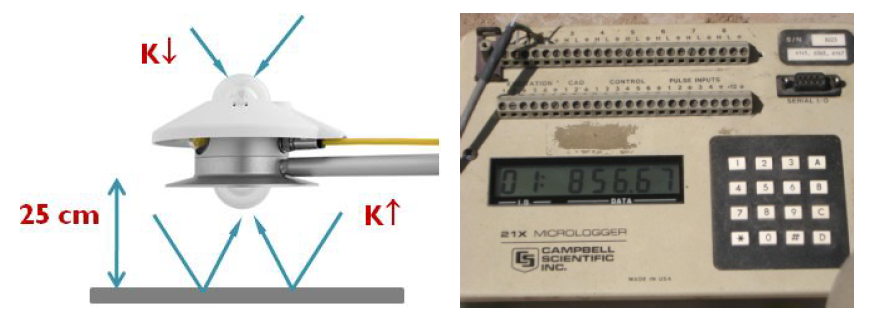
\includegraphics[width=0.9\linewidth]{./figures/measurement-literature/coupled-pyranometer.png}
    \caption{Two coupled-pyranometers (left) and a multi channel data logger}
    \label{fig:albedometer-logger}
\end{figure}

\begin{figure}[!tb]
    \centering
    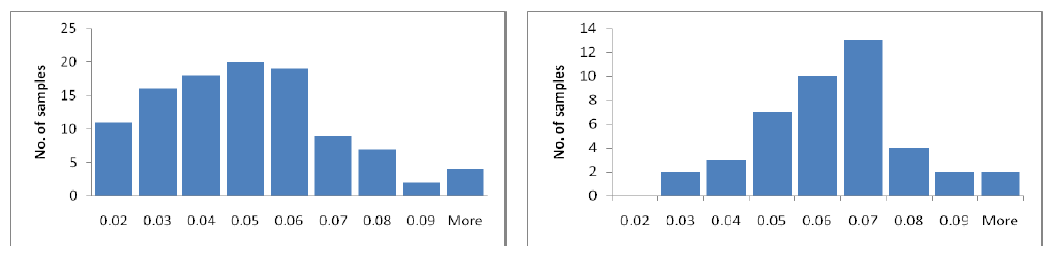
\includegraphics[width=0.9\linewidth]{./figures/measurement-literature/albedo-asphalt-concrete.png}
    \caption{Albedo distribution of 106 asphalt samples (left) and 43 concrete samples (right)}
    \label{fig:albedo-asphalt-concrete}
\end{figure}

A similar albedometer~\cite{2019_Chen} was adapted for the laboratory measurements shown in Fig.\ref{fig:albedometer-lab}, focusing on three asphalt mixtures (Fig.\ref{fig:asphalt-mixture}) and three portland cement concrete (Fig~\ref{fig:pcc}) with different roughness level in the same wavelength range.
In this experimental set-up, the solar radiation was emitted from the infrared lamp with wavelength of $0.3-3\mu m$.
Unlike the field measurements in ~\cite{2011_KUSHARI}, data for incident and reflected radiation were not collected simultaneously.
The lamp and the albedometer were first positioned at the same height above the samples, in order to measure reflected radiation from the lower pyranometer every 30 seconds over a period of 3 minutes.
The final recorded reflected is the mean value of these readings.
Then the albedometer was moved to the position of the sample, and the incident radiation from upper pyranometer was collected.
The asphalt mixture samples were made of crushed basalt aggregate, limestone filler, and modified asphalt, while the Portland cement concrete was made of aggregate, cement, and sand.
Their measured albedo are summarized in Fig.\ref{fig:albedo-pcc-asphalt-mixture}.
We can clearly observe that the later mixture (albedo from $0.228$ to $0.264$) has higher reflectance than the former (albedo $0.0546$ to $0.0611$).
Moreover, the albedo values of the asphalt mixture are consistent with those published in\cite{1988_Blumthaler, 2011_KUSHARI}, providing a reliable reference for future investigations.

\begin{figure}[!tb]
    \centering
    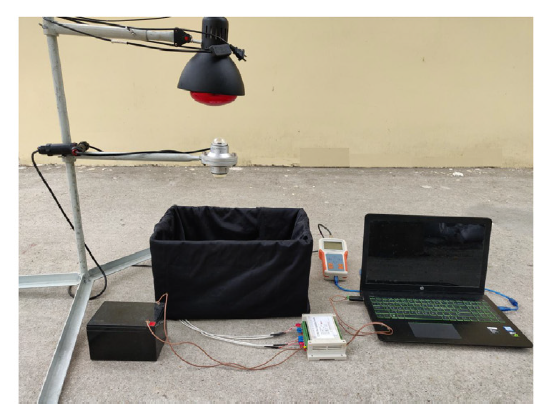
\includegraphics[width=0.8\linewidth]{./figures/measurement-literature/albedometer-lab.png}
    \caption{Albedo lab-based measurement set-up}
    \label{fig:albedometer-lab}
\end{figure}

\begin{figure}[!tb]
    \centering
    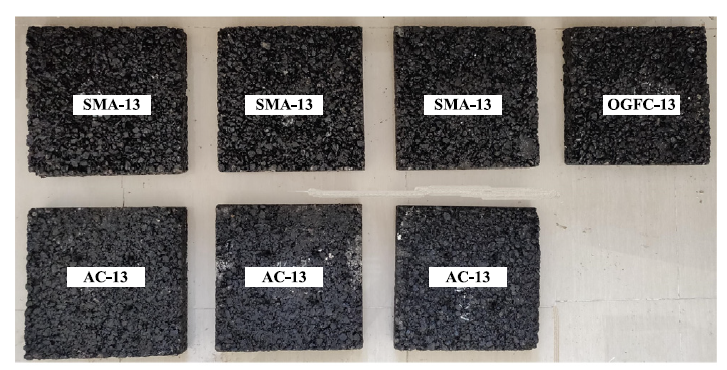
\includegraphics[width=0.8\linewidth]{./figures/measurement-literature/asphalt-mixture.png}
    \caption{3 types of asphalt mixtures}
    \label{fig:asphalt-mixture}
\end{figure}


\begin{figure}[!tb]
    \centering
    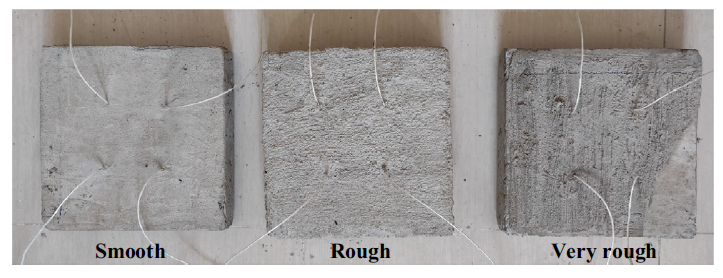
\includegraphics[width=0.8\linewidth]{./figures/measurement-literature/PCC.png}
    \caption{portland cement concrete (PCC)}
    \label{fig:pcc}
\end{figure}

\begin{figure}[!tb]
    \centering
    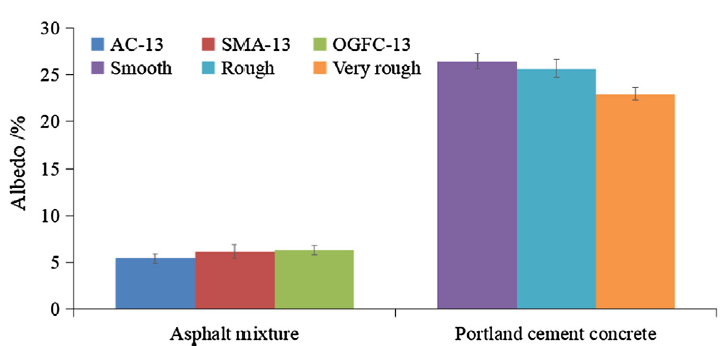
\includegraphics[width=0.8\linewidth]{./figures/measurement-literature/albedo-pcc-asphalt-mixture.png}
    \caption{Albedo of asphalt mixtures and PCC without coating materials}
    \label{fig:albedo-pcc-asphalt-mixture}
\end{figure}
